\begin{figure}[t]
  \centering
   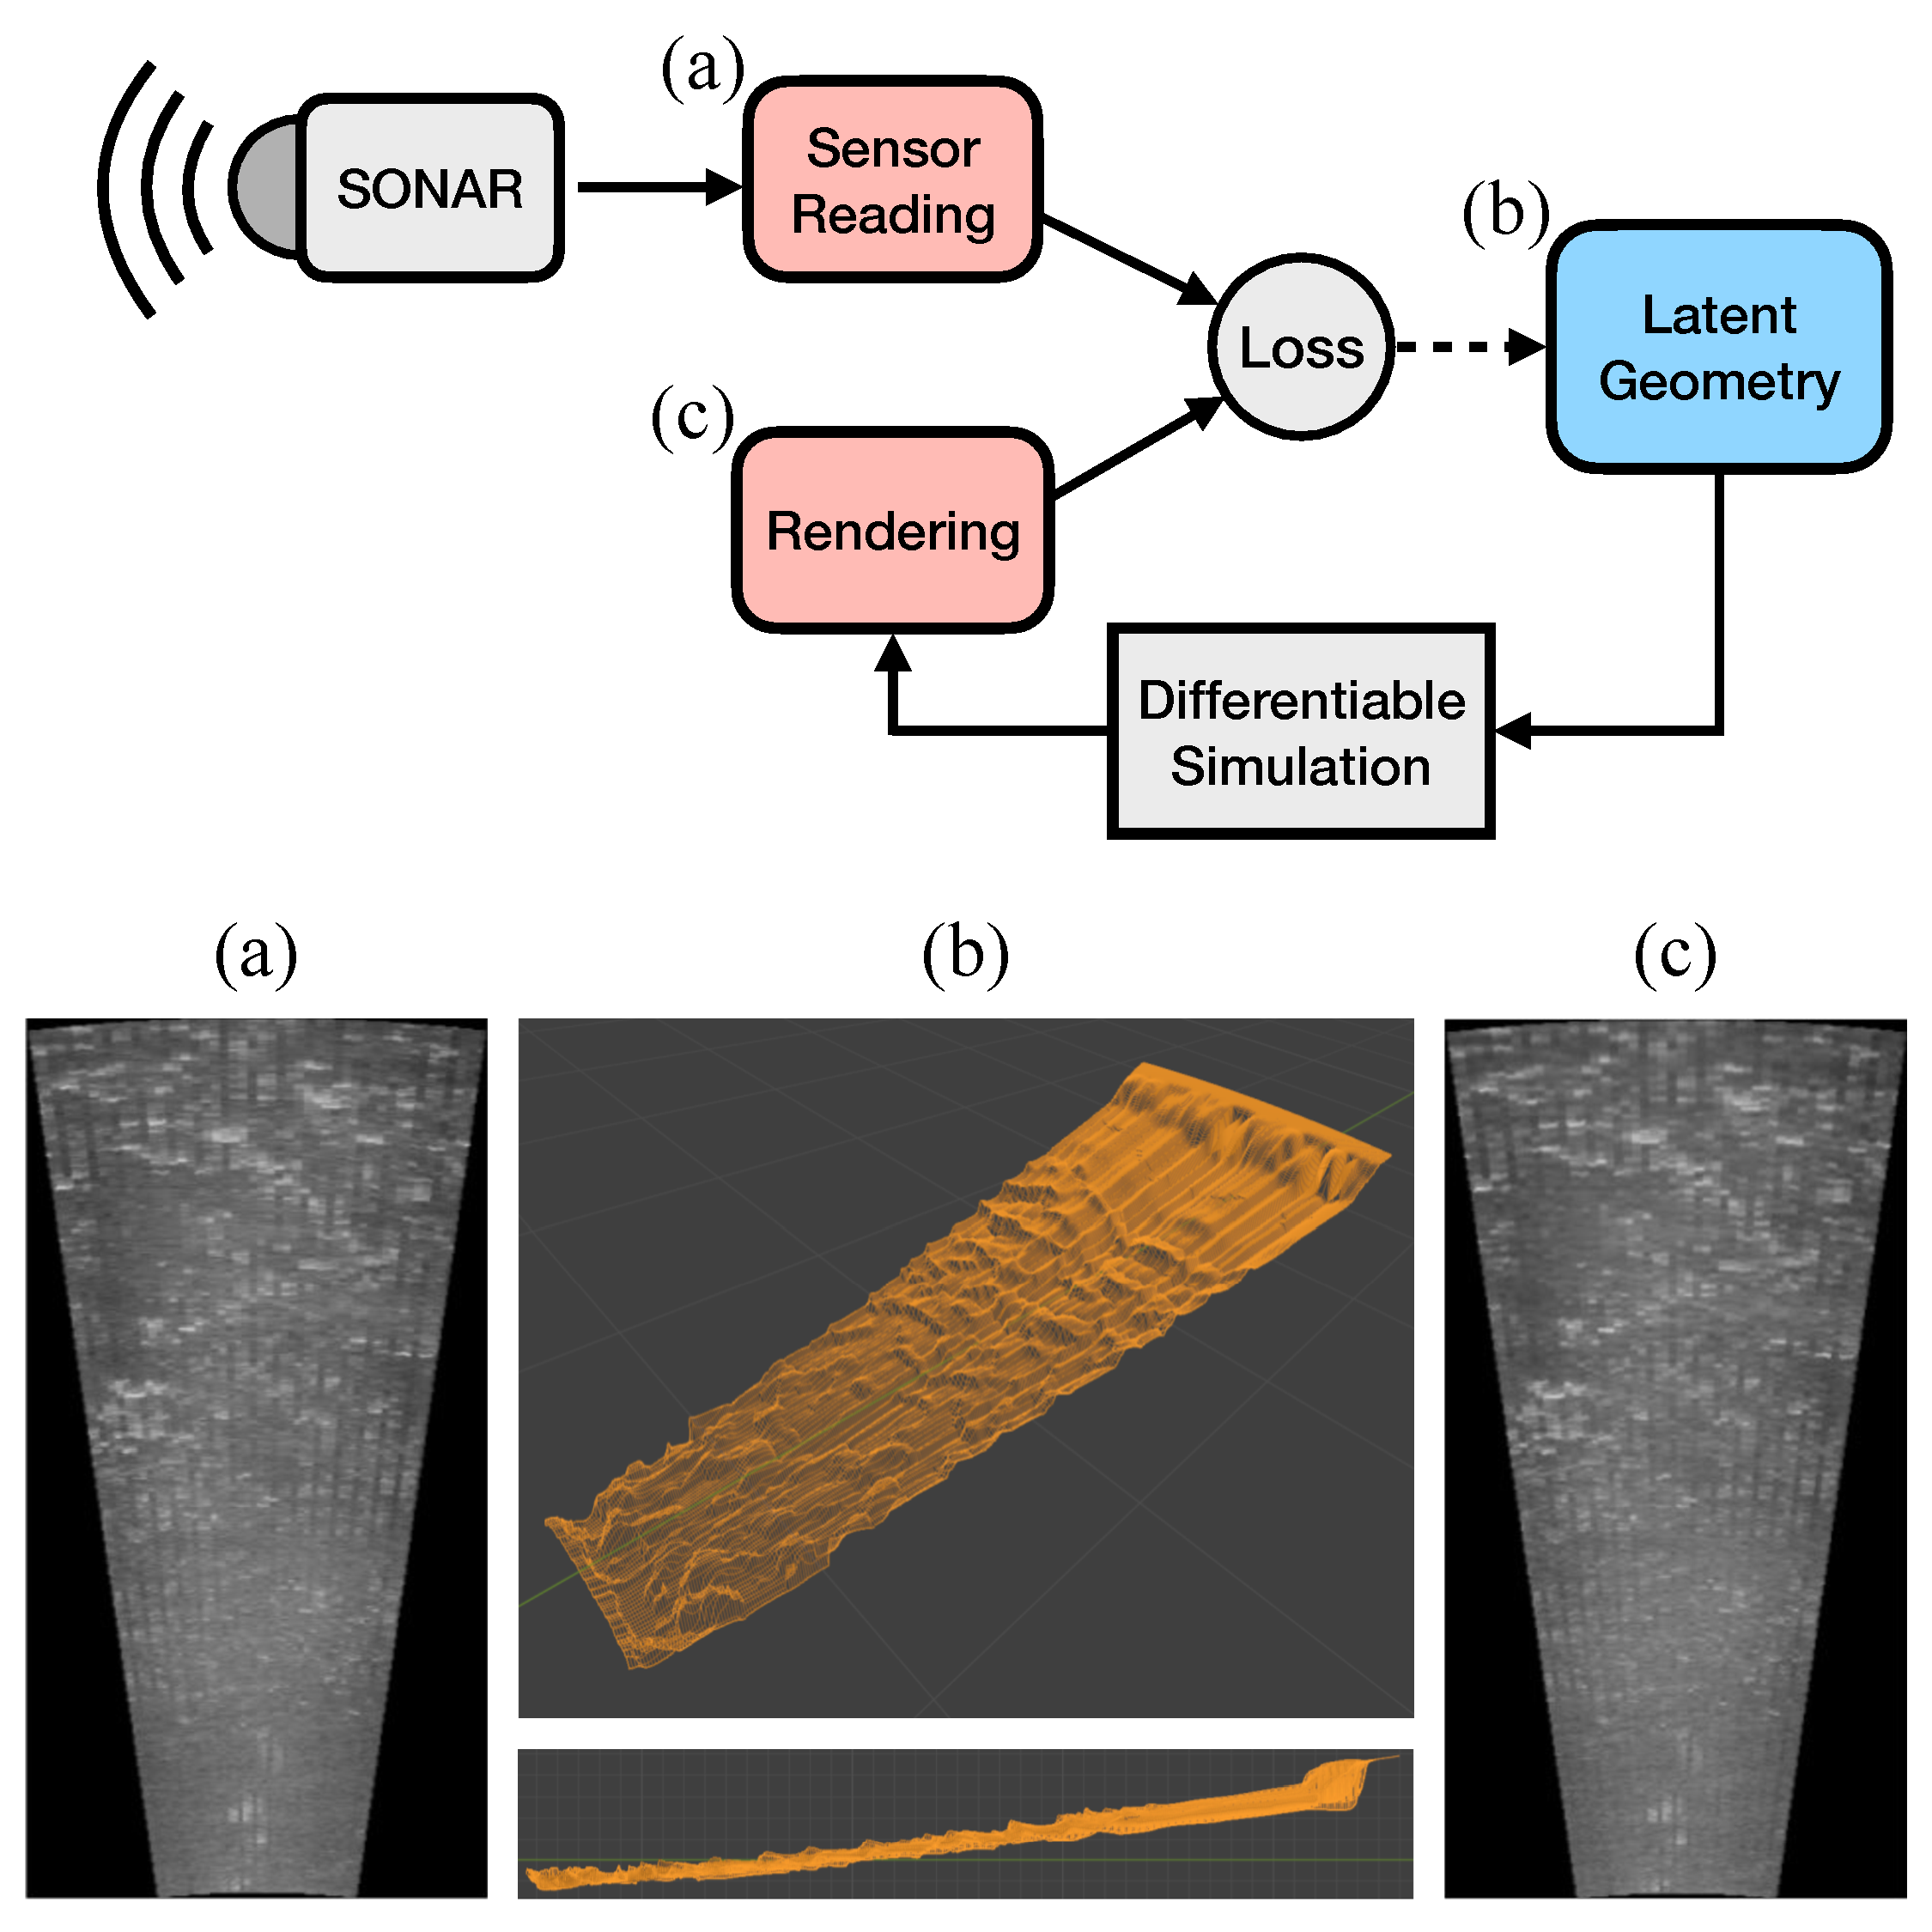
\includegraphics[width=1.0\linewidth]{figs/reconstruction_teaser.pdf}
   \caption{We introduce a differentiable physics simulation of the sonar process which matches a target sensor reading (a) by optimizing a latent height field (b) to minimize the reconstruction error of the simulated output (c) via gradient descent.}
   \label{fig:reconstruction_teaser}
\end{figure}
\section{Introduction}
\label{sec:intro}

Forward-looking sonar (FLS) forms an image by emitting an acoustic pulse into the environment and recording the returned backscatter over angle and time~\cite{Belcher1999DIDSON,Leonard2016AUVNavigation}. It is often the only reliable sensor in underwater settings, with uses including robotics and ecological monitoring. Yet, its images collapse elevation information, producing severe ambiguities, shadows, and noise. For recovering bathymetry, FLS offers advantages for local, short-range environments, \eg mapping a narrow inlet or a confined river segment. 

Multi-view pipelines and sensor fusion can eventually recover elevation from sonar~\cite{Negahdaripour2020FLSGeometry}, but they often require costly deployments, repeated passes, or overlapping sensor coverage. In many field scenarios, including long-term ecological monitoring, practitioners instead rely on a single fixed sonar viewpoint. Being able to infer geometry from a single view enables rapid on-site interpretation, continuous remote observation, and lower system complexity.

Perception-as-generation treats inference as fitting a scene model by simulating candidate states and comparing them to raw sensor measurements. In our setting, the scene is an explicit seafloor height field aligned with the sensor's polar sampling grid. We treat the unknown bathymetry as a latent representation that we iteratively render and refine until the synthetic rendering matches the observed sensor reading. As we explicitly simulate the forward model and parameterize it by real sonar settings, we can adapt to different sensor setups (\eg ranges and beam patterns) while remaining training-free. This gives our system the ability to transfer  readily between settings.
\begin{figure*}[t!]
  \centering
  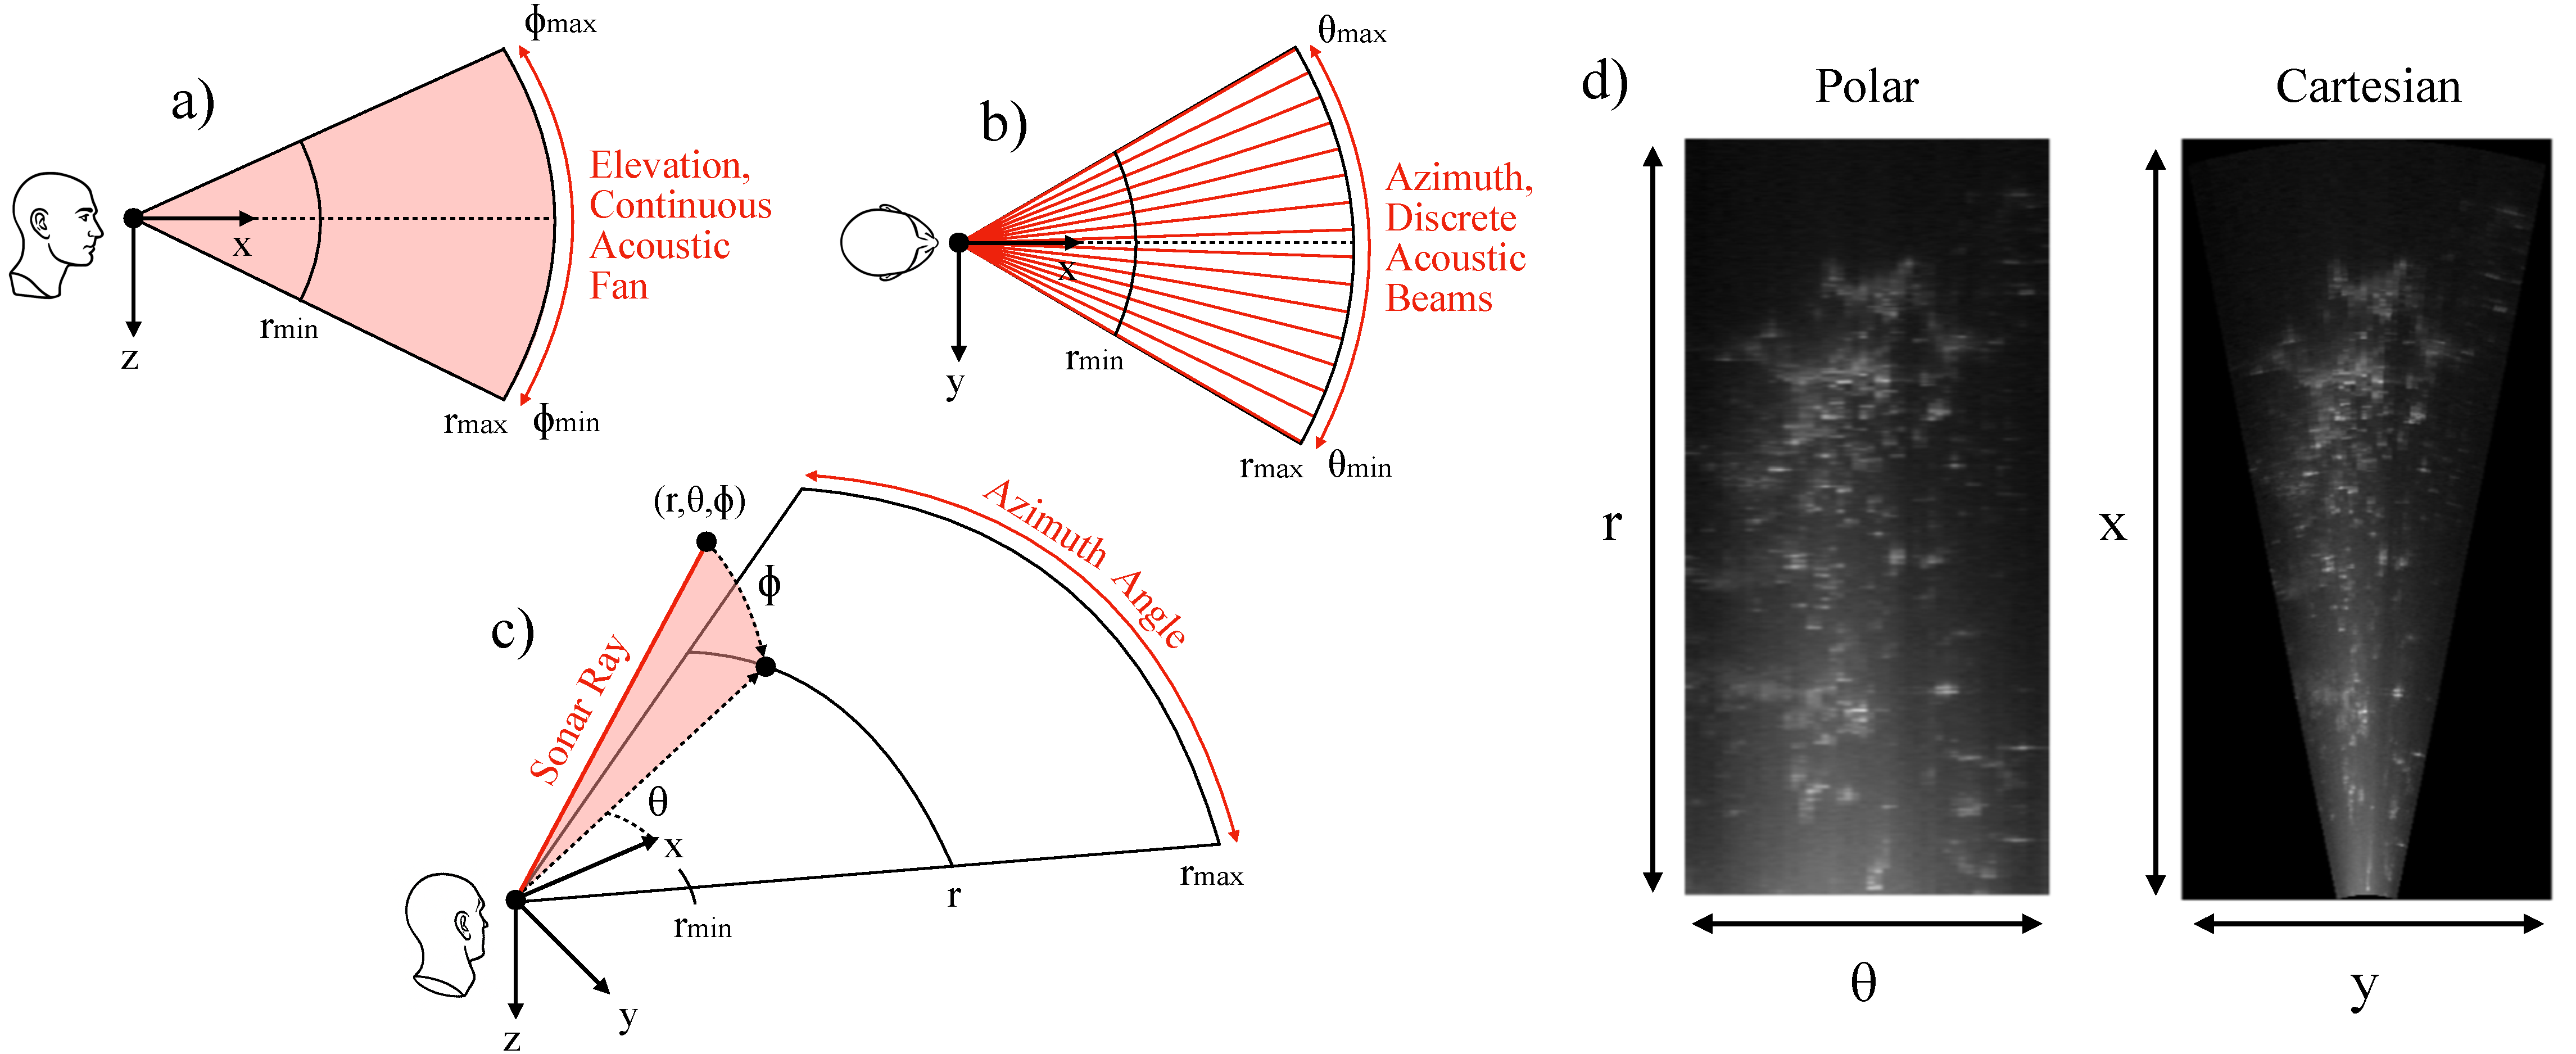
\includegraphics[width=0.95\linewidth]{figs/sonar_overview.pdf}
  \caption{{\bf Overview of the sonar geometric layout from (a) a side view, (b) a top-down view, and (c) an isometric point of view}. As described in Sec.~\ref{sec:imaging_sonar_bg}, the forward-looking sonar (FLS) sampling process can be thought of as a discrete set of azimuthal beams, each comprised of a continuous acoustic signal in the elevation dimension. The signal returns are projected onto the horizontal plane, producing a top-down view of the scene with elevation ambiguity. (d) The sonar image can be viewed in polar coordinates, or warped into Cartesian. In the sonar image, pixel brightness encodes return intensity, while range is determined by the two-way travel time of the acoustic signal.}
  \label{fig:sonar_overview}
  \vspace{-10px}
\end{figure*}

Single-view bathymetry is well-known to be an ill-posed problem since many different scene geometries can explain the same sensor observation. Learning-based approaches, like CNNs, can form priors over a target distribution that allow them to estimate ambiguous geometry, but these priors are not usually invariant to changes in environment or sensor settings. We restrict our focus to settings where the underlying geometry is a height field and ground our reconstruction in principles of sonar physics that translate across domains. {Given the inherent ambiguity of the seafloor tilt in a single FLS view, we focus on recovering geometry conditioned on a known base-plane tilt.}

\vspace{4pt}
\noindent\textbf{Contributions.}
\begin{itemize}[leftmargin=*,nosep]
\item To our knowledge, the first application of differentiable rendering for height recovery in single-view sonar. 
\item A fast, training-free inverse method that optimizes a height field to reconstruct sonar images in \(<\)20 seconds.
\item A method that transfers across sonar configurations and environmental statistics by simulating the physical process with an explicit sensor parameterization. %\red{{More accurate than supervised learning baselines out of distribution.}}
\end{itemize}
